\section{Performance Modeling of the FETI Solvers }

In this section we describe the NUMA effects which significantly affects the performance model, the benchmark problem used for calibration of the model, the approach used for creating the partial models for different blocks of the TFETI and HTFETI solvers and the assembling process of the full model. 

\subsection{NUMA Effect}
\label{sec:numa}
% Processors with architecture Haswell-EP used in Salomon supercomputer (see description in Sec. 
% \ref{sec:salomonDescription}) have 12-core dies. It is designed as it is depicted in Fig. 
% \ref{fig:haswellSocket}, i.e. there are two bi-directional rings in one die. Eight cores with 
% respective slices of L3 cache, QPI interconnect, a memory controller and the PCIe controller are 
% connected to the first ring.


% The remaining four cores with their respective L3 cache slices and the second memory controller 
% are connected to the second bi-directional ring. The rings are then connected together by two 
% queues. Threads from every core can access all DDR4 memory units. It is clear that accessing the local memory, in this case memory on the 
% local ring, is faster, than accessing the remote one (using the memory controller on remote 
% ring). This, so called, \textit{Non-Uniform Memory Access (NUMA)} effect can significantly affect 
% the behavior of parallel applications. 


% This leads us to two types of a possible delay caused by accessing remote memory units. Both types of
% delay are usually called \textit{NUMA effect} and the first type is caused by reading from RAM memory 
% connected closely to the other ring, e.g. accessing DDR4 D memory by thread bounded to the Core 3, 
% considering the Fig. \ref{fig:haswellSocket}. The delay is caused by data transfer through some of the
% queues between the two bi-directional rings.


\begin{figure}[!thb]
\centering
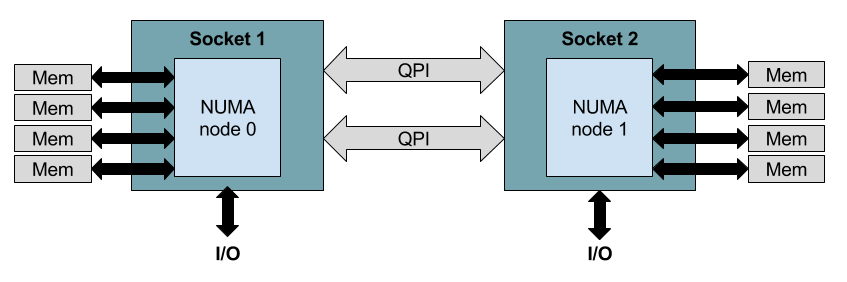
\includegraphics[scale=0.4]{figures/numa.png}
\caption{Dual socket Xeon E5 v3 system - one NUMA node per socket (source \cite{molka2015cache})}
\label{fig:haswellDualSocket}
\end{figure}


%The second and the more significant type of 
The most notable version of the NUMA effect in today HPC clusters is caused by accessing memory attached to another 
socket (i.e.processor) in a multi CPU/socket system. As can be seen from the Fig. \ref{fig:haswellDualSocket}, 
data have to be transferred through the QPI link which decreases the bandwidth and increase the latency of memory transfers. More details about the memory subsystem of the Haswell Xeon CPU can be found in \cite{molka2015cache}.